% Gemini theme
% https://github.com/anishathalye/gemini

\documentclass[final]{beamer}

% ====================
% Packages
% ====================

\usepackage[T1]{fontenc}
\usepackage{lmodern}
\usepackage[size=custom,width=120,height=72,scale=1.0]{beamerposter}
\usetheme{gemini}
\usecolortheme{gemini}
\usepackage{graphicx}
\usepackage{booktabs}
\usepackage{setspace}

% Bibliography setting
\usepackage{paralist}
\usepackage{xpatch}
\usepackage[style=numeric]{biblatex}
\addbibresource{poster.bib}

\usepackage{tikz, pgfplots}

\usetikzlibrary{
    arrows.meta,
    calc,
    decorations,
    decorations.pathreplacing,
    decorations.footprints,
    math,
    patterns,
    shadows,
    external
}

\tikzexternalize

\tikzset{>=stealth}

\pgfplotsset{compat=1.16}

\usepgfplotslibrary{
    polar,
    colormaps,
    colorbrewer,
    groupplots,
    statistics
}

\newcommand{\inputtikz}[1]{%
  \tikzsetnextfilename{#1}%
  \input{#1.tikz}%
}

\newcommand{\doublec}[2]{% double diffusion arrows
  \draw  [-Circle] ($(#1.north east)!0.7!(#1.north)$) -- ($(#2.south east)!0.7!(#2.south)$);
  \draw  [Circle-] ($(#1.north west)!0.7!(#1.north)$) -- ($(#2.south west)!0.7!(#2.south)$);
  }


\newcommand{\singlec}[2]{% single diffusion arrows
  \draw [-Latex] (#1.east) -- (#2.west);
  }

% Set the TikZ neuron style up, since it's used many times
\tikzset{
  neuron/.style={
  % The shape:
  circle,
  % The size:
  minimum size=6mm,
  % The border:
  very thick,
  draw=blue!50!black!50,
  % The filling:
  top color=white,
  bottom color=blue!50!black!20, % and something else at the bottom
  % Font
  font=\itshape,
  % padding around node
  outer sep=2mm
  }
}

\usepackage[siunitx]{circuitikzgit}

\ctikzset{bipoles/length=1cm}

% ====================
% Lengths
% ====================

% If you have N columns, choose \sepwidth and \colwidth such that
% (N+1)*\sepwidth + N*\colwidth = \paperwidth
\newlength{\sepwidth}
\newlength{\colwidth}
\setlength{\sepwidth}{0.025\paperwidth}
\setlength{\colwidth}{0.3\paperwidth}

\newcommand{\separatorcolumn}{\begin{column}{\sepwidth}\end{column}}

% ====================
% Title
% ====================

\title{A minimal reaction-diffusion neural model generates {\emph{C. elegans}} undulation}

\author{Anshul Singhvi \inst{1, 3} \and Harold Hastings \inst{1} \and Jenny Magnes \inst{2} \and Cheris Congo \inst{2} \and Miranda Hulsey-Vincent \inst{2} \and Rifah Tasnim \inst{1} \and Naol Negassa \inst{1}}

\institute[shortinst]{\inst{1} Bard College at Simon's Rock \samelineand \inst{2} Vassar University \samelineand \inst{3} Columbia University}

% ====================
% Footer (optional)
% ====================

\footercontent{
  \href{https://youtu.be/5327kroOwCk}{See the APS March Meeting talk on YouTube} \hfill
  International Physics of Living Systems, 2020 \hfill
  \href{mailto:asinghvi17@simons-rock.edu}{asinghvi17@simons-rock.edu}}
% (can be left out to remove footer)

% ====================
% Logo (optional)
% ====================

% use this to include logos on the left and/or right side of the header:
\logoleft{ 
\includegraphics[width=13cm]{figures/logos/sr.pdf}}
\logoright{
\includegraphics[width=13cm]{figures/logos/vassar.pdf}}


% ====================
% Body
% ====================

\begin{document}

\linespread{1.2}

\begin{frame}[t]
\begin{columns}[t]
\separatorcolumn

\begin{column}{\colwidth}

  \begin{block}{Abstract}

      The small (1 mm) nematode \emph{Caenorhabditis elegans} has become widely used as a model organism; in particular the \emph{C. elegans} connectome has been completely mapped, and \emph{C. elegans} locomotion has been widely studied (c.f. http://www.wormbook.org). We describe a minimal reaction-diffusion model for the \emph{C. elegans}. This may be considered a simple model for Xu et al.'s "descending pathway" description of the \emph{C. elegans} central pattern generator (CPG) \cite{xu2018}. Olivares \emph{et al} \cite{olivares2019} present a likely more realistic model which relies on small networks of neurons, and presents a distributed model of the CPG. In particular, we use simulation methods to show that a small network of FitzHugh-Nagumo neurons (one of the simplest neuronal models) can generate key features of \emph{C. elegans} undulation, and thus locomotion.  Finally, we recreate the required oscillations and coupling with a network of coupled Keener \cite{keener1983} analog neurons.

  \end{block}

\begin{block}{The FitzHugh-Nagumo model}
    The FitzHugh-Nagumo equations have the form:
    \[
    \begin{aligned}
        &\frac{d v}{d t} = f(v) - w + I_{ext} + \color{forestgreen}{D \cdot (v_\mathrm{driving} - v)}\\
        &\frac{d w}{d t} = \epsilon(v - \gamma w + \beta)\\
        &f(v) = v - \frac{v^3}{3}
    \end{aligned}
    \]
    where $v$ is the membrane potential, $w$ is a slow inhibitor variable, AND $\epsilon$, $\gamma$ and $\beta$ are constants.  It turns out that $f(v)$ can be any cubic-like function which sufficiently approximates $v - v^3/3$.
    A method for diffusive inter-neuron coupling has been introduced in green.  $D$ is the diffusion coefficient, and can be positive (excitatory synapses, gap junctions) or negative (inhibitory junctions).  The quantity scaled by $D$ is simply the voltage difference between the driving neuron and the driven one.

\end{block}

  \begin{block}{The central pattern generator}
        A central pattern generator is a small neural circuit which generates and regulates the movement of complex organisms.  This structure is present in different forms in many animals, and it regulates many types of periodic motion.
        \textit{C. elegans} is a small nematode with a well-known neuronal layout.  Its central pattern generator can be sufficiently approximated by a simple neuronal network, arranged as such:The central pattern generator has two principal components.

        \begin{figure}
            \centering
            \inputtikz{figures/cpg/cpg}
            \caption{The central pattern generator, simplified.}
        \end{figure}
        % \begin{minipage}[b]{0.15\pagewidth}
        %     \begin{figure}
        %         \centering
        %         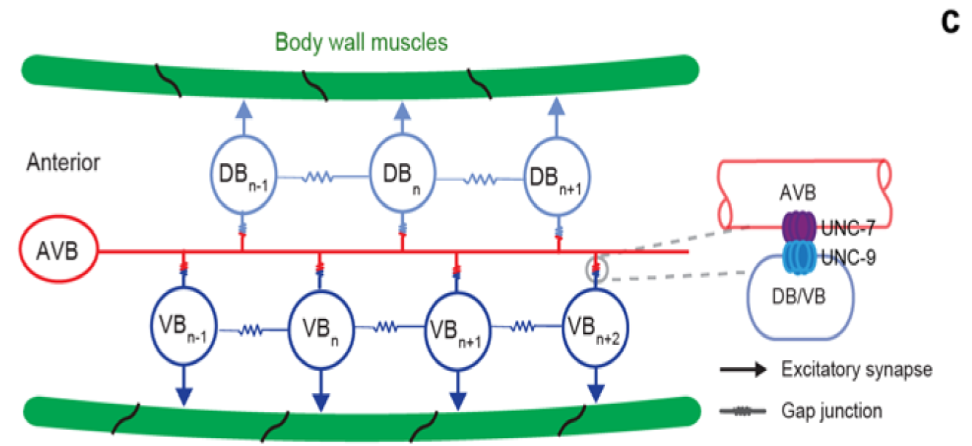
\includegraphics{figures/xu_cpg.png}
        %         \caption{CPG from Xu \textit{et al} \cite{xu2018}.}
        %     \end{figure}
        % \end{minipage}

        wherein \tikz[scale=.68, every node/.style={scale=.6}]{\node (0) [neuron] at (0, 0) {0};\node (1) [neuron] at (3, 0) {1};\draw [-Latex] (0.east) -- (1.west);} represents unidirectional diffusion coupling, and \tikz[scale=.68, every node/.style={scale=.6}]{\node (0) [neuron] at (0, 0) {0}; \node (1) [neuron] at (3, 0) {1}; \draw [-Circle] ($(0.north east)!0.7!(0.east)$) -- ($(1.north west)!0.7!(1.west)$); \draw [Circle-] ($(0.south east)!0.7!(0.east)$) -- ($(1.south west)!0.7!(1.west)$);} represents bidirectional diffusion coupling.  The head oscillator drives the descending pathway to create sinusoidal oscillations.

        % As described by Gjorgjieva \emph{et al} \cite{gjorgjieva2014}, the head oscillator consists of two “head neurons” with mutually inhibitory coupling.  Oscillations are generated when this coupling destabilizes an excitable steady state.
        % This head oscillator then drives a descending pathway, which causes sinusoidal oscillations.

  \end{block}

\end{column}

\separatorcolumn

\begin{column}{\colwidth}

  \begin{block}{Simulation and experimental data}

    \begin{figure}
        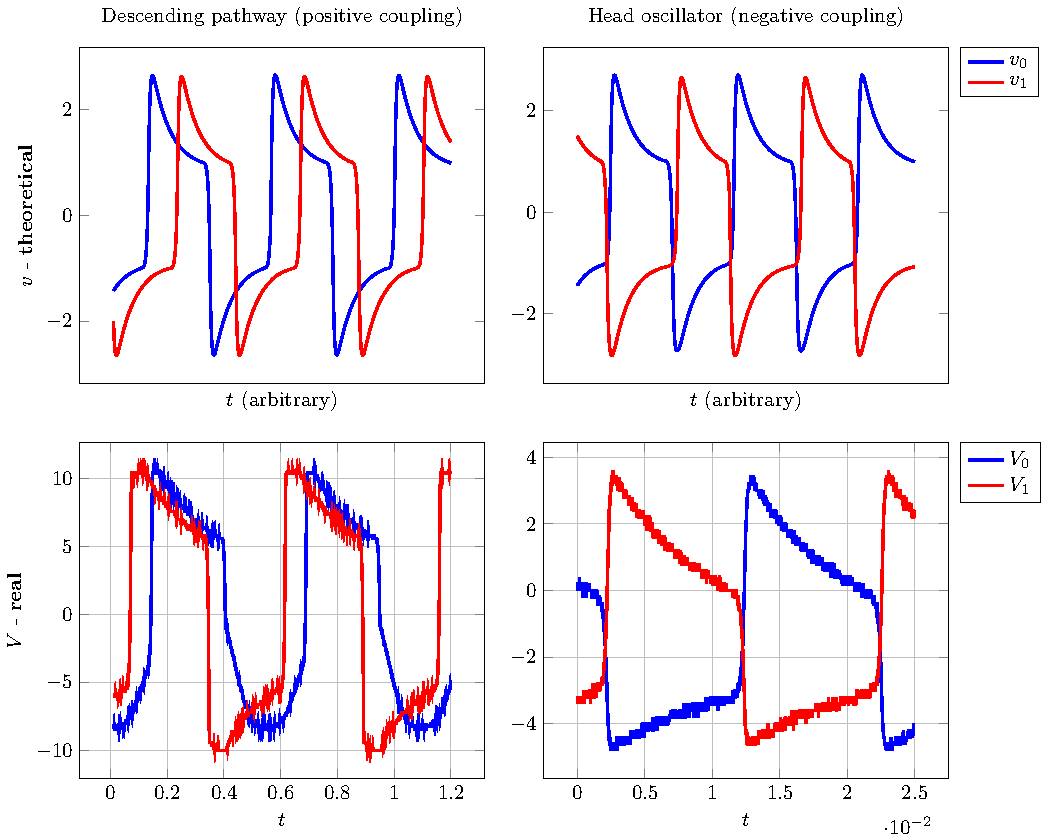
\includegraphics[width=0.9\colwidth]{figures/anal_sim/anal_sim}
        \caption{A comparison between simulation and analog implementation.  Coupled systems of neurons can be used to describe all relevant dynamics of the CPG; in this instance, we use the head oscillator (mutually inhibitory coupling) and a single pair of ventral neurons with positive coupling, to simulate impulse propagation along the descending pathway.}
    \end{figure}

  \end{block}

\end{column}

\separatorcolumn

\begin{column}{\colwidth}

    \begin{block}{The circuit}

    \begin{figure}
        \centering
        \inputtikz{figures/neuron_unit/neuron_unit}
        \caption{Our circuit (modified from \cite{keener1983}), simulating one Keener neuron.}
    \end{figure}

    The FitzHugh-Nagumo equations translate directly into a circuit that uses inductors, as $L = \frac{dI}{dt}$; however, that is an expensive and impractical solution due to mutual inductance effects.  Keener's circuit proposes a simulation of the inductors with operational amplifiers, which make the circuit considerably cheaper and stabler, and allow for a linear piecewise voltage response (from the op-amp) rather than a cubic one (from Nagumo's tunnel diode), resolving the issue of long-term stability.

    The frequency of oscillation changes with the values of the components, as well as the bias voltage, but is approximately $\SI{2}{\hertz}$ with the circuit values here.


    \heading{Coupling}

    We have implemented simple diffusion techniques, using a resistor to vary the coupling strength.  Excitatory (positive-coefficient) coupling is implemented by a simple resistor, whereas inhibitory (negative-coefficient) coupling is implemented by an inverting amplifier, constructed using an operational amplifier and two resistors.

    \begin{figure}
        \centering
        \inputtikz{figures/coupling/coupling}
        \caption{Different inter-neuronal coupling mechanisms.}
    \end{figure}

    \end{block}
    \begin{block}{References}

    \nocite{*}
    \footnotesize{\printbibliography[heading = none]}

    \end{block}

\end{column}

\separatorcolumn
\end{columns}
\end{frame}

\end{document}
